% Backup slides (after \appendix, not counted in the talk).

% ------------------------------------------------------------------------------
\begin{frame}[fragile]{Backup: where the template shortcut comes from}
  \begin{columns}[T]
    \begin{column}{0.42\textwidth}
      \textbf{bad unit}\\[1pt]
\begin{lstlisting}[style=unit]
void sym_0() {
  char *data = NULL;
  data = (char *)malloc(100);
  if (data == NULL) exit(-1);
  strcpy(data, "A String");
  printLine(data);
  ;                  /* no free */
}
\end{lstlisting}
      {\small Function names renamed to \texttt{sym\_N}; abridged.}
    \end{column}
    \begin{column}{0.54\textwidth}
      \textbf{good unit (Original)}\\[1pt]
\begin{lstlisting}[style=unit]
(*\hlc{static void}*) sym_1() {        /* G2B */
  char *data = (char *)ALLOCA(100);
  strcpy(data, "A String"); printLine(data);
}
(*\hlc{static void}*) sym_2() {        /* B2G */
  char *data = (char *)malloc(100);
  ...; printLine(data); free(data);
}
void sym_0() { sym_1(); sym_2(); }
\end{lstlisting}
      {\small Length, function count and \code{static} reveal the label.}
    \end{column}
  \end{columns}
\end{frame}

% ------------------------------------------------------------------------------
\begin{frame}{Backup: task and data}
  \begin{itemize}
    \item One Juliet\sref{sardjuliet13} CWE-401\sref{mitrecwe401} unit (C or C++) $\to$ leak / no leak
    \item 1,658 bad/good groups, 42 families, 48 flow variants
    \item C 868 / C++ 790 groups; 3,316 units per layer
    \item Debiased G2B / B2G good units $\approx$ 50/50 per flow category
    \item Dev 330 groups (9 variants); eval 1,328 groups (39 variants)
  \end{itemize}
\end{frame}

% ------------------------------------------------------------------------------
\begin{frame}{Backup: Original vs Debiased, all detectors}
  \centering
  {\footnotesize\renewcommand{\arraystretch}{0.82}% generated by figures/make_figures.py -- do not edit
\begin{tabular}{@{}lrr@{}}
\toprule
Detector & Original & Debiased \\
\midrule
\alert{\code{static void} $\Rightarrow$ good (probe)} & \alert{1.000} & \alert{0.333} \\
DeepSeek L1 & 0.961$^\dagger$ & 0.995 \\
Jev L1 & 0.956 & 0.971 \\
\textcolor{NeutDraw}{ASan/LSan (ref.)} & \textcolor{NeutDraw}{0.945} & \textcolor{NeutDraw}{0.945} \\
LoRA decision model L1 & 0.943 & 0.984 \\
\alert{grep: no \code{free}/\code{delete} $\Rightarrow$ leak} & \alert{0.935} & \alert{0.701} \\
Clang SA & 0.822 & 0.855 \\
CodeQL & 0.785 & 0.882 \\
Infer & 0.770 & 0.815 \\
Intern-Decision L1 & 0.642 & 0.825 \\
Qwen3.5-4B L1 & 0.572 & 0.754 \\
Cppcheck & 0.467 & 0.493 \\
LineVul & 0.356 & 0.501 \\
\bottomrule
\end{tabular}
}\\[2pt]
  {\scriptsize Macro-F1 on the eval set (2,656 units). $^\dagger$\,DeepSeek: nested25 subset (664 units).
  Tools: Clang SA\sref{clangsa}, Infer\sref{inferpulse}, CodeQL\sref{codeqldocs}, Cppcheck\sref{cppcheck}, LSan\sref{lsan}, LineVul\sref{fu2022linevul}.\par}
\end{frame}

% ------------------------------------------------------------------------------
% src: figures/nearllm.pdf (Debiased eval, v3 figure); bootstrap juliet_full/analysis/near_llm_bootstrap.py
%   (seed 20261123, B=2000): LoRA L1 - DeepSeek L1 = -0.0113 [-0.0143, -0.0084]; latencies figures/latency_c1.csv
%   (Debiased latency300, quiet re-measure); L4-D (opt.) Debiased 0.214 s: juliet_full/l4d_ft/REPORT_stage1.md:137
%   (fallback kernel = prediction config)
\begin{frame}{Backup: on Debiased, the unit-label LoRA was near-cloud}
  \begin{columns}[c]
    \begin{column}{0.58\textwidth}
      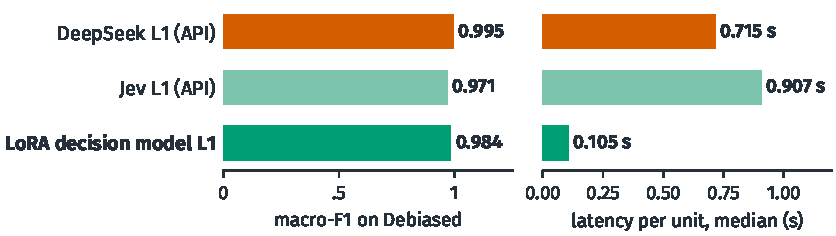
\includegraphics[width=\linewidth]{figures/nearllm.pdf}
    \end{column}
    \begin{column}{0.40\textwidth}
      \small
      \begin{itemize}
        \item LoRA L1 \res{lora_L1-layer1}{macro} vs DeepSeek L1 \res{deepseek_L1-layer1}{macro}: $\Delta$ $-0.011$ $[-0.014, -0.008]$
        \item Debiased latency: 0.105\,s vs 0.715\,s ($\approx$7$\times$)
        \item Same model on DeadFree: \res{df-lora_L1}{macro}
      \end{itemize}
      \vspace{4pt}
      {\scriptsize Debiased latencies (concurrency 1): Clang\sref{clangsa} 0.018, LoRA L1 0.105, Intern\sref{zhu2026interndecision} 0.132, L4-D (opt.) 0.214, Qwen\sref{qwen35card} 0.333, DeepSeek 0.715, Jev 0.907\,s.\par}
    \end{column}
  \end{columns}
\end{frame}

% ------------------------------------------------------------------------------
% src: Debiased/Placebo from registry runs (\res{<key>-<layer>}); DeadFree from deadfree_quality.json (\res{df-<key>});
%   DeepSeek Placebo run is the nested25 subset (664 units)
\begin{frame}{Backup: Placebo control: the guard alone does not hurt}
  \centering
  \small
  \renewcommand{\arraystretch}{1.1}
  \begin{tabular}{@{}lccc@{}}
    \toprule
    Method & Debiased & Placebo (guard, no free) & DeadFree (dead free) \\
    \midrule
    DeepSeek L1 & \res{deepseek_L1-layer1}{macro} & \res{deepseek_L1-placebo}{macro}$^\dagger$ & \res{df-deepseek_L1}{macro} \\
    Jev L3 & \res{jev_L3-layer1}{macro} & \res{jev_L3-placebo}{macro} & \res{df-jev_L3}{macro} \\
    Qwen3.5-4B\sref{qwen35card} L3 & \res{qwen_L3-layer1}{macro} & \res{qwen_L3-placebo}{macro} & \res{df-qwen_L3}{macro} \\
    Intern-Decision\sref{zhu2026interndecision} L3 & \res{intern_L3-layer1}{macro} & \res{intern_L3-placebo}{macro} & \res{df-intern_L3}{macro} \\
    FT L1 (unit labels) & \res{lora_L1-layer1}{macro} & \res{lora_L1-placebo}{macro} & \alert{\res{df-lora_L1}{macro}} \\
    FT L3 (unit labels) & \res{lora_L3-layer1}{macro} & \res{lora_L3-placebo}{macro} & \alert{\res{df-lora_L3}{macro}} \\
    FT L4-D (opt.) & \res{lora_l4d_opt-layer1}{macro} & \res{lora_l4d_opt-placebo}{macro} & \res{df-lora_l4d_opt}{macro} \\
    Clang SA\sref{clangsa} & \res{clang_sa-layer1}{macro} & \res{clang_sa-placebo}{macro} & \res{df-clang_sa}{macro} \\
    grep & \res{grep-layer1}{macro} & \res{grep-placebo}{macro} & \res{df-grep_v0}{macro} \\
    \bottomrule
  \end{tabular}
  \vfill
  {\scriptsize The drop comes from the dead \code{free}, not from the extra branch. $^\dagger$\,nested25 subset (664 units).\par}
\end{frame}

% ------------------------------------------------------------------------------
% src: McNemar rows from report/final_en/tables/res_mcnemar.tex (18 pre-registered tests, Holm);
%   bootstrap rows from juliet_full/analysis/near_llm_bootstrap.py (seed 20261123, B=2000, family-cluster, macro-F1 difference).
\begin{frame}{Backup: paired tests on Debiased (2,656 units)}
  \centering
  \small
  \begin{tabular}{@{}llr@{}}
    \toprule
    A vs B & statistic & result \\
    \midrule
    LoRA L1 vs DeepSeek L1 & $\Delta$macro-F1, 95\% CI & $-0.0113$ $[-0.0143, -0.0084]$ \\
    & only-right units & 12 vs 42 \\
    LoRA L1 vs Jev L1 & $\Delta$macro-F1, 95\% CI & $+0.0132$ $[+0.0029, +0.0282]$ \\
    Intern\sref{zhu2026interndecision} L1 vs Qwen\sref{qwen35card} L1 & $\Delta$macro-F1 & $+0.0711$ \\
    \midrule
    DeepSeek L1 vs DeepSeek L4 & McNemar $b$/$c$, $p_\text{Holm}$ & 63 / 12, $6.2{\times}10^{-8}$ \\
    DeepSeek L1 vs Qwen L1 & McNemar $b$/$c$, $p_\text{Holm}$ & 641 / 0, $9.4{\times}10^{-140}$ \\
    DeepSeek L2 vs CodeQL\sref{codeqldocs} & McNemar $b$/$c$, $p_\text{Holm}$ & 306 / 0, $5.7{\times}10^{-67}$ \\
    \bottomrule
  \end{tabular}
  \vfill
  {\scriptsize Bootstrap: 2,000 family-cluster resamples. McNemar\sref{mcnemar1947}: 18 pre-registered tests, Holm\sref{holm1979}-corrected.\par}
\end{frame}


% ------------------------------------------------------------------------------
% src: juliet_full/analysis/l4d_peek/fact_error_attribution.out.txt via \res{df-x}{attr_layer3_*}
%   (gold facts substituted per question type, rules v1 frozen, eval 2,656 DeadFree units)
\begin{frame}{Backup: fact attribution on DeadFree}
  \centering
  \small
  \renewcommand{\arraystretch}{1.1}
  \begin{tabular}{@{}lccc@{}}
    \toprule
    Gold facts substituted & macro-F1 & FP & FN \\
    \midrule
    none (FT L4-D answers) & \res{df-x}{attr_layer3_none} & \res{df-x}{attr_layer3_none_fp} & \res{df-x}{attr_layer3_none_fn} \\
    \code{heap} & \res{df-x}{attr_layer3_heap} & \res{df-x}{attr_layer3_heap_fp} & \res{df-x}{attr_layer3_heap_fn} \\
    \code{exec\_any} & \res{df-x}{attr_layer3_exec_any} & \res{df-x}{attr_layer3_exec_any_fp} & \res{df-x}{attr_layer3_exec_any_fn} \\
    \code{exec\_all} & \alert{\res{df-x}{attr_layer3_exec_all}} & \res{df-x}{attr_layer3_exec_all_fp} & \res{df-x}{attr_layer3_exec_all_fn} \\
    \code{exec\_any} + \code{exec\_all} & \res{df-x}{attr_layer3_exec_any_exec_all} & \res{df-x}{attr_layer3_exec_any_exec_all_fp} & \res{df-x}{attr_layer3_exec_any_exec_all_fn} \\
    \code{rel} & \res{df-x}{attr_layer3_rel} & \res{df-x}{attr_layer3_rel_fp} & \res{df-x}{attr_layer3_rel_fn} \\
    \code{realloc\_safe} & \res{df-x}{attr_layer3_realloc_safe} & \res{df-x}{attr_layer3_realloc_safe_fp} & \res{df-x}{attr_layer3_realloc_safe_fn} \\
    all (oracle) & \res{df-x}{attr_layer3_all} & \res{df-x}{attr_layer3_all_fp} & \res{df-x}{attr_layer3_all_fn} \\
    \bottomrule
  \end{tabular}
  \vfill
  {\scriptsize Gold \code{rel} removes FNs but not FPs; gold \code{exec\_all} removes both.\par}
\end{frame}

% ------------------------------------------------------------------------------
% src: oracle = \res{df-x}{attr_<layer>_all(_fp|_fn)}; FT = \res{df-x}{attr_<layer>_none}; Original oracle .985:
%   juliet_full/l4d/REPORT_stage1.md:91-97; FPs all flow-variant-12 goods REPORT_stage1.md:102-110
\begin{frame}{Backup: oracle: rules v1 with gold facts}
  \centering
  \small
  \renewcommand{\arraystretch}{1.1}
  \begin{tabular}{@{}lccc@{}}
    \toprule
    & Debiased & DeadFree & Placebo \\
    \midrule
    gold facts (oracle) & \res{df-x}{attr_layer1_all} & \res{df-x}{attr_layer3_all} & \res{df-x}{attr_placebo_all} \\
    \quad FP / FN & \res{df-x}{attr_layer1_all_fp} / \res{df-x}{attr_layer1_all_fn} & \res{df-x}{attr_layer3_all_fp} / \res{df-x}{attr_layer3_all_fn} & \res{df-x}{attr_placebo_all_fp} / \res{df-x}{attr_placebo_all_fn} \\
    FT L4-D answers & \res{df-x}{attr_layer1_none} & \res{df-x}{attr_layer3_none} & \res{df-x}{attr_placebo_none} \\
    \bottomrule
  \end{tabular}
  \vspace{8pt}
  \begin{itemize}
    \item Every oracle error is a false positive on a flow-variant-12 good unit
    \item Variant 12 frees in \emph{both} random branches: each \code{free} has \code{exec\_all} = no, so \code{freed} never fires
    \item ``Some free on every path'' is not expressible with per-statement facts: the ceiling of rules v1
  \end{itemize}
\end{frame}

% ------------------------------------------------------------------------------
% src: juliet_full/l4d_ft/results/scores/lora_l4d_opt_<layer>_eval_r1.json (per_fold, all_eval)
\begin{frame}{Backup: L4-D per held-out fold}
  \centering
  \renewcommand{\arraystretch}{1.1}
  \begin{tabular}{@{}lcccc@{}}
    \toprule
    Layer & fold 0 & fold 1 & fold 2 & pooled \\
    \midrule
    Debiased & \res{df-x}{l4d_layer1_fold0} & \res{df-x}{l4d_layer1_fold1} & \res{df-x}{l4d_layer1_fold2} & \res{df-x}{l4d_layer1} \\
    \textbf{DeadFree} & \res{df-x}{l4d_layer3_fold0} & \res{df-x}{l4d_layer3_fold1} & \res{df-x}{l4d_layer3_fold2} & \textbf{\res{df-x}{l4d_layer3}} \\
    Placebo & \res{df-x}{l4d_placebo_fold0} & \res{df-x}{l4d_placebo_fold1} & \res{df-x}{l4d_placebo_fold2} & \res{df-x}{l4d_placebo} \\
    Original & \res{df-x}{l4d_original_fold0} & \res{df-x}{l4d_original_fold1} & \res{df-x}{l4d_original_fold2} & \res{df-x}{l4d_original} \\
    \bottomrule
  \end{tabular}
  \vfill
  {\scriptsize Each fold's model was trained on the other two folds; checkpoint and $\tau$ chosen on dev and frozen before eval.\par}
\end{frame}

% ------------------------------------------------------------------------------
% src: figures/df_by_flow.tex <- deadfree_quality.json by_flow
\begin{frame}{Backup: DeadFree by flow category}
  \centering
  {\small\resizebox{\linewidth}{!}{% generated by figures/make_figures.py from juliet_full/analysis/deadfree/deadfree_quality.json
\begin{tabular}{@{}lccccc@{}}
\toprule
Method & 01 baseline & 02–22 control flow & 31–45 data flow & 51–68 cross-file & 71–84 C++ objects \\
\midrule
DeepSeek L1 & 0.856 & 0.828 & 0.900 & 0.902 & 0.868 \\
DeepSeek L4 & 0.904 & 0.885 & 0.921 & 0.949 & 0.836 \\
Jev L3 & 0.916 & 0.906 & 0.962 & 0.998 & 0.994 \\
Qwen L3 & 0.893 & 0.836 & 0.769 & 0.703 & 0.457 \\
Intern L3 & 0.748 & 0.612 & 0.657 & 0.776 & 0.605 \\
FT L1 & 0.467 & 0.402 & 0.343 & 0.333 & 0.333 \\
FT L4-D (opt.) & 0.869 & 0.823 & 0.843 & 0.848 & 0.770 \\
Clang SA & 0.904 & 0.868 & 0.827 & 0.923 & 0.691 \\
\bottomrule
\end{tabular}
}\par}
  \vfill
  {\scriptsize Macro-F1 per Juliet\sref{sardjuliet13} flow-variant group, DeadFree eval. FT L1 collapses everywhere; FT L4-D is weakest on C++ objects.\par}
\end{frame}

% ------------------------------------------------------------------------------
% src: figures/df_track_generative.tex, figures/df_track_decision.tex <- deadfree_quality.json (methods.json deadfree.tracks;
%   bold = best cell per row, computed); jev_l4d prints "pending" until its row exists. No L2 for read-out / FT: PLAN.md:35.
\begin{frame}{Backup: two tracks $\times$ four strategies, all numbers}
  \begin{columns}[T]
    \begin{column}{0.47\textwidth}
      {\small\textbf{Generative}: writes text, we parse it}\\[1pt]
      {\footnotesize\setlength{\tabcolsep}{3.5pt}% generated by figures/make_figures.py from juliet_full/analysis/deadfree/deadfree_quality.json
\begin{tabular}{@{}lcccc@{}}
\toprule
 & L1 & L2 & L3 & L4 \\
\midrule
Qwen3.5-4B & 0.533 & 0.595 & \textbf{0.760} & 0.706 \\
\midrule
DeepSeek (cloud) & 0.863 & 0.873 & 0.875 & \textbf{0.900} \\
\bottomrule
\end{tabular}
}
    \end{column}
    \begin{column}{0.51\textwidth}
      {\small\textbf{Decision}: one pass, read P(Yes) vs P(No)}\\[1pt]
      {\footnotesize\setlength{\tabcolsep}{3.5pt}% generated by figures/make_figures.py from juliet_full/analysis/deadfree/deadfree_quality.json
\begin{tabular}{@{}lcccc@{}}
\toprule
 & L1 & L2 & L3 & L4-D \\
\midrule
Qwen read-out & 0.351 & --$^\dagger$ & 0.334 & \textbf{0.752} \\
Intern-Decision & 0.584 & 0.500 & 0.664 & \textbf{0.799} \\
ours (LoRA) & 0.372 & --$^\dagger$ & 0.639 & \textbf{0.826} \\
\midrule
Jev (cloud) & 0.946 & 0.942 & \textbf{0.949} & 0.907 \\
\bottomrule
\end{tabular}
}
    \end{column}
  \end{columns}
  \vfill
  {\scriptsize DeadFree macro-F1; bold = best per row; Jev and Intern at $\tau=0.5$ for every strategy.
  $^\dagger$Not run: FT already saw $\approx$1,800 labelled units; the L2 prompt is 2.4$\times$ longer.\par}
\end{frame}

% ------------------------------------------------------------------------------
% src: figures/df_pareto_full.pdf (same data and front as the main Pareto, every point labelled)
\begin{frame}{Backup: DeadFree Pareto, every point labelled}
  \centering
  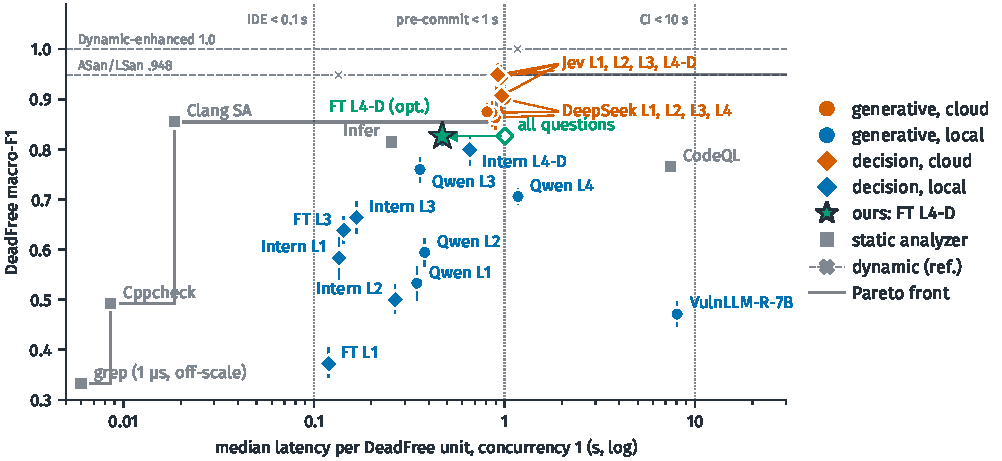
\includegraphics[width=\linewidth,height=0.72\textheight,keepaspectratio]{figures/df_pareto_full.pdf}
  \vfill
  {\scriptsize x: median latency per DeadFree unit, concurrency 1 (log); y: macro-F1 with 95\,\% CI. Front over model-based and static methods.\par}
\end{frame}

% ------------------------------------------------------------------------------
% src: figures/df_strategies.tex <- deadfree_quality.json strategy_x_ft + latency_deadfree.csv
\begin{frame}{Backup: strategy $\times$ local model, macro-F1 / median latency}
  \centering
  {\small\resizebox{\linewidth}{!}{% generated by figures/make_figures.py from juliet_full/analysis/deadfree (quality + latency)
\begin{tabular}{@{}lcccc@{}}
\toprule
Local model & L1 & L2 & L3 & L4 / L4-D \\
\midrule
Qwen3.5-4B (gen.) & 0.533 / {\scriptsize \textit{pending}} & 0.595 / {\scriptsize \textit{pending}} & 0.760 / {\scriptsize \textit{pending}} & 0.706 / {\scriptsize \textit{pending}} \\
Intern-Decision-4B & 0.584 / {\scriptsize \textit{pending}} & 0.500 / {\scriptsize \textit{pending}} & 0.664 / {\scriptsize \textit{pending}} & \textit{pending} / {\scriptsize \textit{pending}} \\
Qwen read-out (no FT) & -- & -- & -- & 0.752 / {\scriptsize \textit{pending}} \\
ours: Qwen3.5-4B + LoRA & 0.372 / {\scriptsize \textit{pending}} & -- & 0.639 / {\scriptsize \textit{pending}} & 0.826 / {\scriptsize 445\,ms} \\
\bottomrule
\end{tabular}
}\par}
  \vfill
  {\scriptsize DeadFree eval, 2,656 units; latency per unit at concurrency 1 on one RTX 3090; n/m = not measured.\par}
\end{frame}

% ------------------------------------------------------------------------------
% src: juliet_full/analysis/deadfree/deadfree_quality.json intern_l4d (tau 0.5, primary), intern_l4d_devtau
%   (dev tau 0.182426, secondary), readout_l4d, paired_deltas; notes[0] (switch after eval), notes[1] (failure)
\begin{frame}{Backup: Intern-Decision L4-D and its threshold}
  \centering
  \renewcommand{\arraystretch}{1.15}
  \begin{tabular}{@{}lcccc@{}}
    \toprule
    Intern-Decision-4B\sref{zhu2026interndecision}, L4-D & macro-F1 [95\,\% CI] & leak P & leak R & gap closed \\
    \midrule
    $\tau = 0.5$ (reported) & \res{df-intern_l4d}{macro} \res{df-intern_l4d}{ci} & \res{df-intern_l4d}{p} & \res{df-intern_l4d}{r} & \res{df-intern_l4d}{gap1} \\
    dev $\tau = 0.18$ (frozen) & \res{df-intern_l4d_devtau}{macro} \res{df-intern_l4d_devtau}{ci} & \res{df-intern_l4d_devtau}{p} & \res{df-intern_l4d_devtau}{r} & \res{df-intern_l4d_devtau}{gap1} \\
    \bottomrule
  \end{tabular}
  \vspace{6pt}
  \begin{itemize}\small
    \item \alert{Disclosure}: the primary was switched to $\tau=0.5$ after seeing eval, for consistency with Intern L1--L3; the switch favours the baseline
    \item Low dev $\tau$: every exec/release question is answered Yes (Intern's $p_{\text{yes}}$ lies in $\approx$0.45--0.65), so dead frees count as ``runs on every path''; a $\tau$ tuned on Debiased (no dead frees) does not transfer
    \item Paired: Intern L4-D $-$ Qwen read-out L4-D \res{df-x}{pd_intern_l4d__readout_l4d} \res{df-x}{pd_intern_l4d__readout_l4d_ci};\\ FT L4-D $-$ Intern L4-D \res{df-x}{pd_lora_l4d_opt__intern_l4d} \res{df-x}{pd_lora_l4d_opt__intern_l4d_ci}
  \end{itemize}
\end{frame}

% ------------------------------------------------------------------------------
% src: deadfree_quality.json jev_l4d (tau 0.5, pre-specified before any call, primary), jev_l4d_devtau (layer1-dev tau
%   0.268941, secondary), paired_deltas; fact accuracy, FP causes and latency protocol:
%   juliet_full/analysis/deadfree/REPORT_jev_l4d.md (eval table, "Reading", per-qtype table, latency table)
\begin{frame}{Backup: Jev L4-D, the cloud decision model on the same facts}
  \centering
  \renewcommand{\arraystretch}{1.15}
  \begin{tabular}{@{}lcccc@{}}
    \toprule
    Jev, L4-D & macro-F1 [95\,\% CI] & leak P & leak R & gap closed \\
    \midrule
    $\tau = 0.5$ (pre-specified) & \res{df-jev_l4d}{macro} \res{df-jev_l4d}{ci} & \res{df-jev_l4d}{p} & \res{df-jev_l4d}{r} & \res{df-jev_l4d}{gap1} \\
    dev-chosen $\tau = 0.27$ & \res{df-jev_l4d_devtau}{macro} \res{df-jev_l4d_devtau}{ci} & \res{df-jev_l4d_devtau}{p} & \res{df-jev_l4d_devtau}{r} & \res{df-jev_l4d_devtau}{gap1} \\
    \bottomrule
  \end{tabular}
  \vspace{6pt}
  \begin{itemize}\small
    \item Same pruned questions and rules as Intern and FT L4-D; $\tau = 0.5$ fixed before any Jev L4-D call
    \item Paired: vs DeepSeek L4 \res{df-x}{pd_jev_l4d__deepseek_L4} \res{df-x}{pd_jev_l4d__deepseek_L4_ci} (n.s.);
      vs Jev L3 \res{df-x}{pd_jev_l4d__jev_L3} \res{df-x}{pd_jev_l4d__jev_L3_ci};\\ vs FT L4-D \res{df-x}{pd_jev_l4d__lora_l4d_opt} \res{df-x}{pd_jev_l4d__lora_l4d_opt_ci}
    \item \code{exec\_all} fact accuracy 0.975 (FT L4-D 0.831): a strong decision model answers path questions well;
      most of its 238 false leaks contain a wrong \code{realloc\_safe} answer
    \item Latency \res{df-jev_l4d}{lat}: the questions of a unit are sent concurrently (local L4-D asks them one by one)
  \end{itemize}
\end{frame}

% ------------------------------------------------------------------------------
% src: deadfree_quality.json vulnllmr; configuration juliet_full/STATUS.md 2026-11-23 22:41 (authors' prompt with
%   policy hint CWE-401/1333/703/404, #judge: yes = leak, unparseable = wrong)
\begin{frame}{Backup: VulnLLM-R-7B, a vulnerability-reasoning model}
  \begin{itemize}
    \item VulnLLM-R-7B\sref{nie2025vulnllmr}: authors' prompt and policy hint (CWE-401, 1333, 703, 404); temperature 0
    \item DeadFree: macro-F1 \res{df-vulnllmr}{macro} \res{df-vulnllmr}{ci}
    \item Leak precision \res{df-vulnllmr}{p}, recall \res{df-vulnllmr}{r} (TP \res{df-vulnllmr}{tp}, FN \res{df-vulnllmr}{fn})
    \item Below both untuned 4B models on DeadFree
  \end{itemize}
  \vfill
  {\scriptsize ``\#judge: yes'' with any type = leak; unparseable or truncated output counts as wrong.\par}
\end{frame}

% ------------------------------------------------------------------------------
% src: prompts juliet_full/llm/prompts (frozen on dev); L4-D templates juliet_full/l4d/templates.py (TEMPLATE_SHA256,
%   frozen), abridged only by dropping the code snippet in backticks
\begin{frame}{Backup: prompts and the five L4-D question templates}
  \footnotesize
  \begin{description}[L4-D]
    \item[L1] unit code $\to$ \code{\{label, confidence\}}; decision models read P(leak)
    \item[L2] + fixed dev examples (few-shot)
    \item[L3] + Clang SA\sref{clangsa} warnings for the unit
    \item[L4] LLM lists \code{alloc/free/assign/call/dead(line)} facts as JSON; Souffl\'e\sref{jordan2016souffle} \code{leak.dl} decides
    \item[L4-D] one yes/no question per fact, statement under test masked as \code{\_\_TARGET\_\_();}
  \end{description}
  {\scriptsize
  \begin{tabular}{@{}lp{0.76\linewidth}@{}}
    \toprule
    \code{heap} & Does the call at line \{line\} allocate heap memory that the program must release? \\
    \code{exec\_any} & Can the statement at line \{line\} execute on at least one run of the program? \\
    \code{exec\_all} & Does the statement at line \{line\} execute on every run of the program? \\
    \code{rel} & Does the release at line \{line\_f\} free the block obtained at line \{line\_a\}? \\
    \code{realloc\_safe} & If the realloc at line \{line\} fails and returns NULL, is the original block still released later? \\
    \bottomrule
  \end{tabular}\par}
  \vfill
  {\scriptsize Same prompt text for all models; temperature 0, thinking off; frozen before eval.\par}
\end{frame}

% ------------------------------------------------------------------------------
% src: juliet_full/l4d/l4d.dl (rules v1, comments dropped)
\begin{frame}[fragile]{Backup: L4-D rules v1 (Souffl\'e, complete)}
\begin{lstlisting}[style=dl]
.input unit, alloc, realloc, heap, exec_any, exec_all, rel, realloc_safe
heap_block(u, a) :- alloc(u, a), heap(u, a).
heap_block(u, r) :- realloc(u, r).
freed(u, a) :- rel(u, f, a), exec_all(u, f).
leak(u, a, "never_freed")  :- heap_block(u, a), exec_any(u, a), !freed(u, a).
leak(u, r, "realloc_fail") :- realloc(u, r), exec_any(u, r), !realloc_safe(u, r).
unit_leak(u) :- leak(u, _, _).
.output leak, unit_leak
\end{lstlisting}
  \vspace{4pt}
  \begin{itemize}\small
    \item \code{alloc}, \code{realloc}: site lists from the tree-sitter\sref{url-treesitter} parser; all other inputs: model answers with $p \geq \tau$
    \item Frozen before training; refinements were allowed only from Debiased dev failures (there were none)
  \end{itemize}
\end{frame}

% ------------------------------------------------------------------------------
% src: juliet_full/llm/l4/leak.dl (v3 L4 rules, abridged); numbers from registry runs (DeepSeek DeadFree = nested25)
\begin{frame}[fragile]{Backup: L4 (LLM facts + Datalog), the v3 rule set}
  \begin{columns}[T]
    \begin{column}{0.59\textwidth}
\begin{lstlisting}[style=dl]
reach("main").
reach(g) :- reach(f), call(f, g, l), !dead(l).
new_obj(o, v, f) :- alloc(o, v, f, l),
                    reach(f), !dead(l).
pts(s, v, o) :- new_obj(o, v, f),
                scope(f, v, s).
pts(sd, d, o) :- assign(d, x, f, l), !dead(l),
                 ..., pts(sx, x, o).
freed(o) :- free(v, f, l), reach(f), !dead(l),
            ..., pts(s, v, o).
(*\textcolor{OIblue}{\bfseries leak(o, "never\_freed")}*) :-
        new_obj(o, _, _), !freed(o).
\end{lstlisting}
      {\tiny Abridged from \texttt{juliet\_full/llm/l4/leak.dl} (v3): Andersen-style, flow-insensitive;
      + \texttt{realloc\_fail} rule.\par}
    \end{column}
    \begin{column}{0.39\textwidth}
      \begin{itemize}\small
        \item DeepSeek L4, Debiased: \res{deepseek_L4-layer1}{macro} (L1 \res{deepseek_L1-layer1}{macro})
        \item DeadFree $\Delta$ \res{deepseek_L4-layer3}{d}, smallest of L1--L4 (L1 \res{deepseek_L1-layer3}{d})
        \item FP/FN: L1 \res{deepseek_L1-layer3}{fp}/\res{deepseek_L1-layer3}{fn},
              L4 \res{deepseek_L4-layer3}{fp}/\res{deepseek_L4-layer3}{fn}
        \item 99.87\% of facts grounded to a source line
        \item Qwen3.5-4B L4: \res{qwen_L4-layer1}{macro} $\to$ \res{qwen_L4-layer3}{macro}
      \end{itemize}
    \end{column}
  \end{columns}
  \vfill
  {\scriptsize Paired on nested25 (664 units). A dead \code{free} is dropped by \code{!dead(l)}, so the leak survives.\par}
\end{frame}


% ------------------------------------------------------------------------------
\begin{frame}{Backup: method matrix with versions}
  \footnotesize
  \renewcommand{\arraystretch}{0.9}
  \begin{tabular}{@{}lll@{}}
    \toprule
    Group & Method & Program-analysis idea \\
    \midrule
    Static & grep: is there a \code{free}/\code{delete}? & lexical baseline \\
           & Cppcheck\sref{cppcheck} 2.22 & intraprocedural dataflow \\
           & Clang SA\sref{clangsa} 23.1.6 & path-sensitive symbolic execution \\
           & CodeQL\sref{codeqldocs} 2.27.5 & Datalog-style queries over dataflow \\
           & Infer\sref{inferpulse} 1.3 (Pulse) & interprocedural summaries \\
    Generative & DeepSeek V4.1 Flash (API) $\times$ L1--L4 & L4: LLM facts + Datalog \\
        & Qwen3.5-4B (local) $\times$ L1--L4 & same prompts, one RTX 3090 \\
        & VulnLLM-R-7B\sref{nie2025vulnllmr} (local) & authors' reasoning prompt \\
    Decision & Jev (TypeSafe API) $\times$ L1--L3 & read the option probability \\
             & Intern-Decision-4B $\times$ L1--L3 (+ L4-D) & read the option probability \\
             & Qwen3.5-4B read-out $\times$ L4-D & untuned Yes/No head \\
             & \textbf{ours}: LoRA $\times$ \{L1, L3, L4-D\} & fine-tuned score, 3-fold CV \\
    \midrule
    \textcolor{NeutDraw}{Reference} & \textcolor{NeutDraw}{ASan/LSan\sref{lsan}, Valgrind\sref{nethercote2007valgrind}, Dynamic-enhanced} &
      \textcolor{NeutDraw}{runs the program: shown, not ranked} \\
    \bottomrule
  \end{tabular}
  \vfill
  {\scriptsize Missing output, timeout or compile error counts as a wrong prediction.\par}
\end{frame}

% ------------------------------------------------------------------------------
% src: figures/cost.tex <- juliet_full/llm/ledger.jsonl; per-1k cost report/final_en/generated/numbers.tex
%   (res-x-cost1k_deepseek_L1, res-x-cost1k_jev_L1); FT cost juliet_full/l4d_ft/PROGRESS.md:8
\begin{frame}{Backup: cost of every API run and of fine-tuning}
  \begin{columns}[T]
    \begin{column}{0.60\textwidth}
      {\scriptsize\resizebox{\linewidth}{!}{% generated by figures/make_figures.py from juliet_full/llm/ledger.jsonl
\begin{tabular}{@{}llrr@{}}
\toprule
Provider & Runs & calls & cost \\
\midrule
DeepSeek & Debiased (incl.\ dev, repeats, latency) & 13,877 & \textyen5.46 \\
DeepSeek & DeadFree & 11,824 & \textyen5.37 \\
DeepSeek & Placebo & 1,328 & \textyen0.42 \\
DeepSeek & Original & 664 & \textyen0.30 \\
DeepSeek & demo & 30 & \textyen0.01 \\
\textbf{DeepSeek} & \textbf{total} & \textbf{27,723} & \textbf{\textyen11.57} \\
\midrule
Jev & Debiased (incl.\ dev, repeats, latency) & 27,420 & \$1.23 \\
Jev & DeadFree & 8,868 & \$0.42 \\
Jev & Placebo & 5,312 & \$0.20 \\
Jev & Original & 2,656 & \$0.10 \\
Jev & demo & 11 & \$0.00 \\
\textbf{Jev} & \textbf{total} & \textbf{44,267} & \textbf{\$1.95} \\
\bottomrule
\end{tabular}
}\par}
    \end{column}
    \begin{column}{0.37\textwidth}
      \begin{itemize}\small
        \item Total: \textyen\res{x}{cost_deepseek} and \$\res{x}{cost_jev}
        \item Per 1k units: DeepSeek L1 \textyen0.397, Jev L1 \$0.0345
        \item L4-D fine-tuning: $\approx$68\,min per fold on 2$\times$ RTX 3090 ($\approx$2.3\,GPU-h)
        \item Local inference: no API cost
      \end{itemize}
    \end{column}
  \end{columns}
\end{frame}

% ------------------------------------------------------------------------------
\begin{frame}{Backup: Debiased latency at concurrency 1 (v3 measurements)}
  \centering
  {\tiny\renewcommand{\arraystretch}{0.92}\resizebox{\linewidth}{!}{% generated by figures/make_figures.py from figures/latency_c1.csv
\begin{tabular}{@{}lrl@{}}
\toprule
Method & s / unit & Source (juliet\_full/\ldots); note \\
\midrule
grep & <0.001 & \texttt{static/results/grep\_v0/layer1/lat300\_c1.jsonl}; median of 300 units (1 µs) \\
Cppcheck & 0.008 & \texttt{static\_stage2.md}; lat300 per unit \\
Clang SA & 0.018 & \texttt{static\_stage2.md}; lat300 per unit \\
Infer & 0.278 & \texttt{static\_stage2.md}; lat300 per unit \\
CodeQL & 7.36 & \texttt{static\_stage2.md}; per unit: database creation + queries (20 units) \\
CodeQL (50 per database) & 0.318 & \texttt{static\_stage2.md}; 50 units per database; amortized (hollow marker) \\
LineVul (GPU) & 0.006 & \texttt{gpu\_stage1.md}; GPU (RTX 3090) \\
LineVul (CPU) & 0.088 & \texttt{gpu/results/linevul\_cpu/layer1/lat300\_cpu\_quiet.jsonl}; CPU 6 threads; quiet; median of 300 \\
DeepSeek L1 & 0.721 & \texttt{llm\_stage2b.md}; lat300\_c1\_L1 at load ~21; quiet 0.640 s on 30 dev units (llm\_stage2a) \\
Qwen L1 & 0.665 & \texttt{gpu\_stage1.md}; vLLM from dell; 30 requests \\
Jev L1 & 0.961 & \texttt{llm\_stage2b.md}; lat300\_c1\_L1 at load ~22 \\
Intern-D L1 & 0.083 & \texttt{gpu\_stage1.md}; /decide read-out from dell (82.7 ms) \\
LoRA L1 & 0.105 & \texttt{decision\_ft\_stage2.md}; latency300; dell end-to-end \\
LoRA L3 & 0.133 & \texttt{decision\_ft\_stage2.md}; latency300; dell end-to-end \\
ASan/LSan & 0.134 & \texttt{data\_stage4.md}; lat300\_c1; compile included \\
Valgrind & 0.407 & \texttt{data\_stage4.md}; lat300\_c1; compile included \\
Dyn. enhanced & 1.194 & \texttt{data\_stage4.md}; lat300\_c1; compile included \\
\bottomrule
\end{tabular}
}\par}
  \vfill
  {\scriptsize Measured on \textbf{Debiased} units; the DeadFree latencies in the main slides are re-measured separately.
  Source table: \texttt{figures/latency\_c1.csv}.\par}
\end{frame}

% ------------------------------------------------------------------------------
\begin{frame}{Backup: are the labels still right? Compile and run every unit}
  \begin{columns}[T]
    \begin{column}{0.46\textwidth}
      \begin{itemize}\small
        \item gcc and clang compile \textbf{3,316 / 3,316} units in every layer
        \item No good unit flagged by ASan\sref{serebryany2012asan}/LSan\sref{lsan} or Dynamic-enhanced
        \item Labels never changed; disagreements explained
      \end{itemize}
    \end{column}
    \begin{column}{0.51\textwidth}
      {\footnotesize Dynamic-enhanced: what it takes to catch the 1,658 bad units\\[2pt]
      \begin{tabular}{@{}lr@{}}
        \toprule
        Needed & units \\
        \midrule
        plain run, every seed & 1,448 \\
        some seeds only (variant 12, random) & 34 \\
        \texttt{use\_globals=0} (globals at exit) & 68 \\
        \texttt{realloc} failure injected & 108 \\
        \bottomrule
      \end{tabular}}
    \end{column}
  \end{columns}
\end{frame}


% ------------------------------------------------------------------------------
% src: deadfree_quality.json asan_lsan / dynamic_enhanced; misses juliet_full/lane_reports data_stage4 (v3 backup)
\begin{frame}{Backup: dynamic analysis is a reference line, not a competitor}
  \begin{itemize}
    \item ASan\sref{serebryany2012asan}/LSan\sref{lsan} on DeadFree: precision \res{df-asan_lsan}{p}, macro-F1 \res{df-asan_lsan}{macro}
    \item Misses: \code{realloc} failure; globals at exit; random branch not taken
    \item Dynamic-enhanced (coverage via gcov\sref{url-gcov}, trace, failure injection): \res{df-dynamic_enhanced}{macro}; we chose inputs and faults
    \item Needs a build, a run and the right input; the same machinery labels the L4-D training facts
  \end{itemize}
\end{frame}

% ------------------------------------------------------------------------------
\begin{frame}{Backup: demo, all detectors on the stage unit}
  \centering
  {\footnotesize% generated by figures/make_figures.py from presentation/demo/recordings/stage_final_v2.json
\begin{tabular}{@{}lccc r@{}}
\toprule
Detector & bad & good twin & bad + dead free & ms \\
\midrule
grep & \cmark\,leak & \cmark\,no leak & \xmark\,no leak\,\textcolor{OIvermil}{\small flipped} & 2 \\
Clang SA & \cmark\,leak & \cmark\,no leak & \cmark\,leak & 191 \\
old LoRA L1 (unit labels) & \cmark\,leak & \cmark\,no leak & \xmark\,no leak\,\textcolor{OIvermil}{\small flipped} & 378 \\
old LoRA L3 (unit labels) & \cmark\,leak & \cmark\,no leak & \xmark\,no leak\,\textcolor{OIvermil}{\small flipped} & 760 \\
FT L4-D (opt.) & \cmark\,leak & \cmark\,no leak & \cmark\,leak & 223 \\
DeepSeek L1 & \cmark\,leak & \cmark\,no leak & \cmark\,leak & 887 \\
DeepSeek L3 & \cmark\,leak & \cmark\,no leak & \cmark\,leak & 1209 \\
Jev L1 & \cmark\,leak & \cmark\,no leak & \cmark\,leak & 948 \\
\bottomrule
\end{tabular}
\par}
  \vfill
  {\scriptsize Fallback: \texttt{demo.py --replay recordings/\res{x}{demo_file}}. Dry-run cost: \textyen\res{x}{demo_cny} DeepSeek, \$\res{x}{demo_usd} Jev.\par}
\end{frame}

% ------------------------------------------------------------------------------
\begin{frame}{Backup: DeadFree result files}
  \footnotesize
  \begin{itemize}
    \item Quality, CIs, $\Delta$ and gap closed: \texttt{juliet\_full/analysis/deadfree/deadfree\_quality.json}
    \item Latency (median, p90, hardware): \texttt{juliet\_full/analysis/deadfree/latency\_deadfree.csv}
    \item L4-D answers: \texttt{juliet\_full/l4d\_ft/results/lora\_l4d\_opt/<layer>/eval\_r1\_units.jsonl}
    \item Pruning check: \texttt{juliet\_full/l4d\_ft/results/scores/prune\_test.json}
    \item Fact attribution: \texttt{juliet\_full/analysis/l4d\_peek/fact\_error\_attribution.out.txt}
    \item Probes: \texttt{juliet\_full/data/build/probes\_layer3.json}
  \end{itemize}
  \vfill
  {\scriptsize All slide numbers come from \texttt{figures/make\_figures.py}; missing values print as \textit{pending}.\par}
\end{frame}

% ------------------------------------------------------------------------------
% generated by figures/make_figures.py -- do not edit (input outside a frame)
\begin{frame}{Backup: result files used (1/5)}
\centering
{\tiny\renewcommand{\arraystretch}{0.85}\setlength{\tabcolsep}{4pt}\begin{tabular}{@{}llll@{}}
\toprule
Method & Layer & Run file (juliet\_full/\ldots; r = results) & sha256 \\
\midrule
grep & Debiased & \texttt{static/r/grep\_v0/layer1/full\_v1.jsonl} & \texttt{9a425c0e} \\
grep & DeadFree & \texttt{static/r/grep\_v0/layer3/full\_v1.jsonl} & \texttt{a0a26ccd} \\
grep & Placebo & \texttt{static/r/grep\_v0/placebo/full\_v1.jsonl} & \texttt{0e7c92ed} \\
grep & Original & \texttt{static/r/grep\_v0/original/full\_v1.jsonl} & \texttt{5c3bf9ea} \\
Cppcheck & Debiased & \texttt{static/r/cppcheck/layer1/full\_v2.jsonl} & \texttt{b3ae0a0e} \\
Cppcheck & DeadFree & \texttt{static/r/cppcheck/layer3/full\_v1.jsonl} & \texttt{3bd521e3} \\
Cppcheck & Placebo & \texttt{static/r/cppcheck/placebo/full\_v1.jsonl} & \texttt{aade3fed} \\
Cppcheck & Original & \texttt{static/r/cppcheck/original/full\_v1.jsonl} & \texttt{26245ae1} \\
Clang SA & Debiased & \texttt{static/r/clang\_sa/layer1/full\_v2.jsonl} & \texttt{9fff5bc7} \\
Clang SA & DeadFree & \texttt{static/r/clang\_sa/layer3/full\_v1.jsonl} & \texttt{29c2c3cb} \\
Clang SA & Placebo & \texttt{static/r/clang\_sa/placebo/full\_v1.jsonl} & \texttt{a031bf11} \\
Clang SA & Original & \texttt{static/r/clang\_sa/original/full\_v1.jsonl} & \texttt{d48a49c1} \\
CodeQL & Debiased & \texttt{static/r/codeql/layer1/full\_batch50\_merged.jsonl} & \texttt{1e41db0c} \\
CodeQL & DeadFree & \texttt{static/r/codeql/layer3/full\_batch50.jsonl} & \texttt{26cf528a} \\
CodeQL & Placebo & \texttt{static/r/codeql/placebo/full\_batch50.jsonl} & \texttt{203de4f7} \\
CodeQL & Original & \texttt{static/r/codeql/original/full\_batch50.jsonl} & \texttt{e6133458} \\
Infer & Debiased & \texttt{static/r/infer/layer1/full\_per\_file\_merged.jsonl} & \texttt{ba59f70d} \\
Infer & DeadFree & \texttt{static/r/infer/layer3/full\_per\_file.jsonl} & \texttt{69dda662} \\
Infer & Placebo & \texttt{static/r/infer/placebo/full\_per\_file.jsonl} & \texttt{161f789c} \\
Infer & Original & \texttt{static/r/infer/original/full\_per\_file.jsonl} & \texttt{36074229} \\
LineVul & Debiased & \texttt{gpu/r/linevul\_gpu/layer1/deveval\_v1.jsonl} & \texttt{8bc1535e} \\
LineVul & DeadFree & \texttt{gpu/r/linevul\_gpu/layer3/all\_v1.jsonl} & \texttt{2bf0d6ab} \\
\bottomrule
\end{tabular}\par}
\vfill
{\scriptsize Scored with \texttt{juliet\_full/analysis/score.py} on the eval set (2,656 units); \texttt{figures/make\_figures.py}.\par}
\end{frame}
\begin{frame}{Backup: result files used (2/5)}
\centering
{\tiny\renewcommand{\arraystretch}{0.85}\setlength{\tabcolsep}{4pt}\begin{tabular}{@{}llll@{}}
\toprule
Method & Layer & Run file (juliet\_full/\ldots; r = results) & sha256 \\
\midrule
LineVul & Placebo & \texttt{gpu/r/linevul\_gpu/placebo/all\_v1.jsonl} & \texttt{19529812} \\
LineVul & Original & \texttt{gpu/r/linevul\_gpu/original/all\_v1.jsonl} & \texttt{7d2e9b26} \\
ASan/LSan & Debiased & \texttt{data/r/asan\_lsan/layer1/full\_v1.jsonl} & \texttt{684c4195} \\
ASan/LSan & DeadFree & \texttt{data/r/asan\_lsan/stress/full\_v1.jsonl} & \texttt{97a9eb40} \\
ASan/LSan & Placebo & \texttt{data/r/asan\_lsan/placebo/full\_v1.jsonl} & \texttt{9eda685e} \\
ASan/LSan & Original & \texttt{data/r/asan\_lsan/original/full\_v1.jsonl} & \texttt{8945394e} \\
Valgrind & Debiased & \texttt{data/r/valgrind/layer1/full\_v1.jsonl} & \texttt{fb6481b7} \\
Dynamic-enhanced & Debiased & \texttt{data/r/dynamic\_enhanced/layer1/full\_v1.jsonl} & \texttt{758daeac} \\
Dynamic-enhanced & DeadFree & \texttt{data/r/dynamic\_enhanced/stress/full\_v1.jsonl} & \texttt{cf47c76c} \\
Dynamic-enhanced & Placebo & \texttt{data/r/dynamic\_enhanced/placebo/full\_v1.jsonl} & \texttt{181e81b2} \\
DeepSeek L1 & Debiased & \texttt{llm/r/deepseek\_flash/layer1/eval\_L1\_r1.jsonl} & \texttt{912db2f0} \\
DeepSeek L1 & DeadFree & \texttt{llm/r/deepseek\_flash/layer3/l3\_n25\_L1\_r1.jsonl} & \texttt{376d1393} \\
DeepSeek L1 & Placebo & \texttt{llm/r/deepseek\_flash/placebo/pl\_n25\_L1\_r1.jsonl} & \texttt{6480450e} \\
DeepSeek L1 & Original & \texttt{llm/r/deepseek\_flash/original/orig\_n25\_L1\_r1.jsonl} & \texttt{034fdebe} \\
DeepSeek L2 & Debiased & \texttt{llm/r/deepseek\_flash/layer1/eval\_L2\_r1.jsonl} & \texttt{ee6c51f4} \\
DeepSeek L2 & DeadFree & \texttt{llm/r/deepseek\_flash/layer3/l3\_n25\_L2\_r1.jsonl} & \texttt{369a2a1f} \\
DeepSeek L3 & Debiased & \texttt{llm/r/deepseek\_flash/layer1/eval\_L3\_r1.jsonl} & \texttt{4bf6db11} \\
DeepSeek L3 & DeadFree & \texttt{llm/r/deepseek\_flash/layer3/l3\_n25\_L3\_r1.jsonl} & \texttt{6f396914} \\
DeepSeek L3 & Placebo & \texttt{llm/r/deepseek\_flash/placebo/pl\_n25\_L3\_r1.jsonl} & \texttt{c56b0f67} \\
DeepSeek L4 & Debiased & \texttt{llm/r/deepseek\_flash/layer1/eval\_L4\_r1.jsonl} & \texttt{0af89897} \\
DeepSeek L4 & DeadFree & \texttt{llm/r/deepseek\_flash/layer3/l3\_n25\_L4\_r1.jsonl} & \texttt{37d32759} \\
Qwen3.5-4B L1 & Debiased & \texttt{llm/r/qwen3\_5\_4b/layer1/eval\_L1\_r1.jsonl} & \texttt{0c952905} \\
\bottomrule
\end{tabular}\par}
\vfill
{\scriptsize Scored with \texttt{juliet\_full/analysis/score.py} on the eval set (2,656 units); \texttt{figures/make\_figures.py}.\par}
\end{frame}
\begin{frame}{Backup: result files used (3/5)}
\centering
{\tiny\renewcommand{\arraystretch}{0.85}\setlength{\tabcolsep}{4pt}\begin{tabular}{@{}llll@{}}
\toprule
Method & Layer & Run file (juliet\_full/\ldots; r = results) & sha256 \\
\midrule
Qwen3.5-4B L1 & DeadFree & \texttt{llm/r/qwen3\_5\_4b/layer3/l3\_eval\_L1\_r1.jsonl} & \texttt{c9e21163} \\
Qwen3.5-4B L1 & Placebo & \texttt{llm/r/qwen3\_5\_4b/placebo/pl\_eval\_L1\_r1.jsonl} & \texttt{41998d19} \\
Qwen3.5-4B L1 & Original & \texttt{llm/r/qwen3\_5\_4b/original/orig\_eval\_L1\_r1.jsonl} & \texttt{d0a08dbd} \\
Qwen3.5-4B L2 & Debiased & \texttt{llm/r/qwen3\_5\_4b/layer1/eval\_L2\_r1.jsonl} & \texttt{43c641b2} \\
Qwen3.5-4B L2 & DeadFree & \texttt{llm/r/qwen3\_5\_4b/layer3/l3\_eval\_L2\_r1.jsonl} & \texttt{337dc906} \\
Qwen3.5-4B L3 & Debiased & \texttt{llm/r/qwen3\_5\_4b/layer1/eval\_L3\_r1.jsonl} & \texttt{d0d1469a} \\
Qwen3.5-4B L3 & DeadFree & \texttt{llm/r/qwen3\_5\_4b/layer3/l3\_eval\_L3\_r1.jsonl} & \texttt{3c3ddd18} \\
Qwen3.5-4B L3 & Placebo & \texttt{llm/r/qwen3\_5\_4b/placebo/pl\_eval\_L3\_r1.jsonl} & \texttt{9fdeb3fd} \\
Qwen3.5-4B L4 & Debiased & \texttt{llm/r/qwen3\_5\_4b/layer1/eval\_L4\_r1.jsonl} & \texttt{266a3cc9} \\
Qwen3.5-4B L4 & DeadFree & \texttt{llm/r/qwen3\_5\_4b/layer3/l3\_eval\_L4\_r1.jsonl} & \texttt{5c2708a1} \\
Jev L1 & Debiased & \texttt{llm/r/jev/layer1/eval\_L1\_r1.jsonl} & \texttt{b0a4576e} \\
Jev L1 & DeadFree & \texttt{llm/r/jev/layer3/l3\_eval\_L1\_r1.jsonl} & \texttt{59fe6079} \\
Jev L1 & Placebo & \texttt{llm/r/jev/placebo/pl\_eval\_L1\_r1.jsonl} & \texttt{77d9bfce} \\
Jev L1 & Original & \texttt{llm/r/jev/original/orig\_eval\_L1\_r1.jsonl} & \texttt{6d574be5} \\
Jev L2 & Debiased & \texttt{llm/r/jev/layer1/eval\_L2\_r1.jsonl} & \texttt{ca0bf9e1} \\
Jev L2 & DeadFree & \texttt{llm/r/jev/layer3/l3\_eval\_L2\_r1.jsonl} & \texttt{fbe5242d} \\
Jev L3 & Debiased & \texttt{llm/r/jev/layer1/eval\_L3\_r1.jsonl} & \texttt{a5977265} \\
Jev L3 & DeadFree & \texttt{llm/r/jev/layer3/l3\_eval\_L3\_r1.jsonl} & \texttt{cb498e82} \\
Jev L3 & Placebo & \texttt{llm/r/jev/placebo/pl\_eval\_L3\_r1.jsonl} & \texttt{f5c6f04e} \\
Intern-Decision L1 & Debiased & \texttt{gpu/r/intern\_decision/layer1/eval\_L1\_r1.jsonl} & \texttt{f1e87ff7} \\
Intern-Decision L1 & DeadFree & \texttt{gpu/r/intern\_decision/layer3/l3\_eval\_L1\_r1.jsonl} & \texttt{7a52bf2f} \\
Intern-Decision L1 & Placebo & \texttt{gpu/r/intern\_decision/placebo/pl\_eval\_L1\_r1.jsonl} & \texttt{a784841c} \\
\bottomrule
\end{tabular}\par}
\vfill
{\scriptsize Scored with \texttt{juliet\_full/analysis/score.py} on the eval set (2,656 units); \texttt{figures/make\_figures.py}.\par}
\end{frame}
\begin{frame}{Backup: result files used (4/5)}
\centering
{\tiny\renewcommand{\arraystretch}{0.85}\setlength{\tabcolsep}{4pt}\begin{tabular}{@{}llll@{}}
\toprule
Method & Layer & Run file (juliet\_full/\ldots; r = results) & sha256 \\
\midrule
Intern-Decision L1 & Original & \texttt{gpu/r/intern\_decision/original/orig\_eval\_L1\_r1.jsonl} & \texttt{84f4bd18} \\
Intern-Decision L2 & Debiased & \texttt{gpu/r/intern\_decision/layer1/eval\_L2\_r1.jsonl} & \texttt{3feb32b2} \\
Intern-Decision L2 & DeadFree & \texttt{gpu/r/intern\_decision/layer3/l3\_eval\_L2\_r1.jsonl} & \texttt{37419c78} \\
Intern-Decision L3 & Debiased & \texttt{gpu/r/intern\_decision/layer1/eval\_L3\_r1.jsonl} & \texttt{9251594a} \\
Intern-Decision L3 & DeadFree & \texttt{gpu/r/intern\_decision/layer3/l3\_eval\_L3\_r1.jsonl} & \texttt{01ea2eb7} \\
Intern-Decision L3 & Placebo & \texttt{gpu/r/intern\_decision/placebo/pl\_eval\_L3\_r1.jsonl} & \texttt{b5be8128} \\
LoRA decision model L1 & Debiased & \texttt{decision\_ft/r/decision\_ft/layer1/L1\_cv\_v1.jsonl} & \texttt{82f901e2} \\
LoRA decision model L1 & DeadFree & \texttt{decision\_ft/r/decision\_ft/layer3/L1\_cv\_v1.jsonl} & \texttt{797bb4bb} \\
LoRA decision model L1 & Placebo & \texttt{decision\_ft/r/decision\_ft/placebo/L1\_cv\_v1.jsonl} & \texttt{123ddefc} \\
LoRA decision model L1 & Original & \texttt{decision\_ft/r/decision\_ft/original/L1\_cv\_v1.jsonl} & \texttt{3bf56a58} \\
LoRA decision model L3 & Debiased & \texttt{decision\_ft/r/decision\_ft/layer1/L3\_cv\_v1.jsonl} & \texttt{d76d94b9} \\
LoRA decision model L3 & DeadFree & \texttt{decision\_ft/r/decision\_ft/layer3/L3\_cv\_v1.jsonl} & \texttt{903680f7} \\
LoRA decision model L3 & Placebo & \texttt{decision\_ft/r/decision\_ft/placebo/L3\_cv\_v1.jsonl} & \texttt{d52fa746} \\
L4-D decision model (opt.) & Debiased & \texttt{l4d\_ft/r/lora\_l4d\_opt/layer1/eval\_r1\_units.jsonl} & \texttt{87791590} \\
L4-D decision model (opt.) & DeadFree & \texttt{l4d\_ft/r/lora\_l4d\_opt/layer3/eval\_r1\_units.jsonl} & \texttt{3409d5cc} \\
L4-D decision model (opt.) & Placebo & \texttt{l4d\_ft/r/lora\_l4d\_opt/placebo/eval\_r1\_units.jsonl} & \texttt{16edbdfa} \\
L4-D decision model (opt.) & Original & \texttt{l4d\_ft/r/lora\_l4d\_opt/original/eval\_r1\_units.jsonl} & \texttt{206a3089} \\
No-LoRA read-out L1 & Debiased & \texttt{decision\_ft/r/qwen\_readout\_zeroshot/layer1/L1\_v1.jsonl} & \texttt{cac9ab4c} \\
No-LoRA read-out L1 & DeadFree & \texttt{decision\_ft/r/qwen\_readout\_zeroshot/layer3/L1\_v1.jsonl} & \texttt{64ee4b28} \\
LoRA decision model L1 unmerged & Debiased & \texttt{decision\_ft/r/decision\_ft/layer1/unmerged\_L1\_fold0\_v1.jsonl (+2)} & \texttt{23d377ec} \\
No-LoRA read-out L3 & Debiased & \texttt{decision\_ft/r/qwen\_readout\_zeroshot/layer1/L3\_v1.jsonl} & \texttt{72bf7f18} \\
No-LoRA read-out L3 & DeadFree & \texttt{decision\_ft/r/qwen\_readout\_zeroshot/layer3/L3\_v1.jsonl} & \texttt{f738465d} \\
\bottomrule
\end{tabular}\par}
\vfill
{\scriptsize Scored with \texttt{juliet\_full/analysis/score.py} on the eval set (2,656 units); \texttt{figures/make\_figures.py}.\par}
\end{frame}
\begin{frame}{Backup: result files used (5/5)}
\centering
{\tiny\renewcommand{\arraystretch}{0.85}\setlength{\tabcolsep}{4pt}\begin{tabular}{@{}llll@{}}
\toprule
Method & Layer & Run file (juliet\_full/\ldots; r = results) & sha256 \\
\midrule
LoRA decision model L3 unmerged & Debiased & \texttt{decision\_ft/r/decision\_ft/layer1/unmerged\_L3\_fold0\_v1.jsonl (+2)} & \texttt{0ed06f4f} \\
\bottomrule
\end{tabular}\par}
\vfill
{\scriptsize Scored with \texttt{juliet\_full/analysis/score.py} on the eval set (2,656 units); \texttt{figures/make\_figures.py}.\par}
\end{frame}

